\documentclass[border=4pt]{standalone}
\usepackage{tikz}
\usepackage{pgfplots}
\pgfplotsset{compat=1.18}
\usetikzlibrary{shapes.geometric,arrows.meta,positioning,fit,calc,decorations.pathreplacing}
\usepackage{xcolor}
\definecolor{bestcol}{HTML}{1565C0}
\definecolor{freegreen}{HTML}{2E7D32}
\definecolor{learnblue}{HTML}{1565C0}
\definecolor{fusred}{HTML}{C62828}
\newcommand{\best}[1]{{\color{bestcol}\textbf{#1}}}
\begin{document}
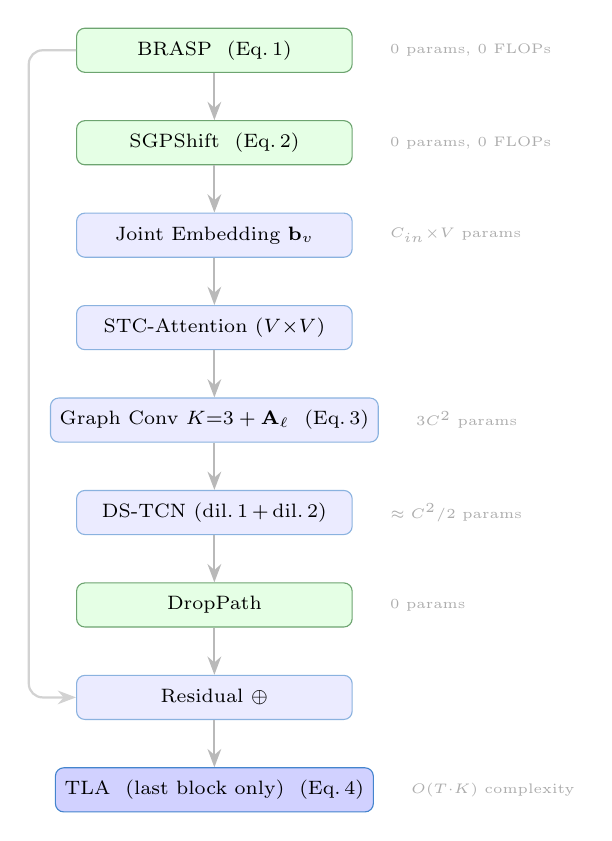
\begin{tikzpicture}[
  every node/.style={font=\scriptsize},
  box/.style={draw, rounded corners=3pt, minimum width=3.5cm,
              minimum height=0.56cm, align=center},
  free/.style={box, fill=green!10, draw=freegreen!70},
  learn/.style={box, fill=blue!8,  draw=learnblue!50},
  hilit/.style={box, fill=blue!18, draw=learnblue!80},
  ann/.style={font=\tiny, text=gray!65, anchor=west},
  arr/.style={-Stealth, thick, draw=gray!55},
  skip/.style={-Stealth, thick, draw=gray!35, rounded corners=5pt}
]
\node[free]  (brasp) at (0,0)      {BRASP\ \ (Eq.\,1)};
\node[free, below=0.60cm of brasp] (sgp)   {SGPShift\ \ (Eq.\,2)};
\node[learn, below=0.60cm of sgp]  (je)    {Joint Embedding $\mathbf{b}_v$};
\node[learn, below=0.60cm of je]   (stca)  {STC-Attention ($V{\times}V$)};
\node[learn, below=0.60cm of stca] (gcn)   {Graph Conv $K{=}3 + \mathbf{A}_\ell$\ \ (Eq.\,3)};
\node[learn, below=0.60cm of gcn]  (tcn)   {DS-TCN\ (dil.\,1\,+\,dil.\,2)};
\node[free, below=0.60cm of tcn]   (dp)    {DropPath};
\node[learn, below=0.60cm of dp]   (res)   {Residual $\oplus$};
\node[hilit, below=0.60cm of res]  (tla)   {TLA\ \ (last block only)\ \ (Eq.\,4)};

%% skip
\draw[skip] (brasp.west) -- +(-0.6,0) |- (res.west);

\foreach \a/\b in {brasp/sgp,sgp/je,je/stca,stca/gcn,gcn/tcn,tcn/dp,dp/res,res/tla}
  \draw[arr] (\a)--(\b);

%% annotations right
\node[ann, right=0.35cm of brasp] {0 params, 0 FLOPs};
\node[ann, right=0.35cm of sgp]   {0 params, 0 FLOPs};
\node[ann, right=0.35cm of je]    {$C_\text{in}{\times}V$ params};
\node[ann, right=0.35cm of gcn]   {$3C^2$ params};
\node[ann, right=0.35cm of tcn]   {$\approx C^2/2$ params};
\node[ann, right=0.35cm of dp]    {0 params};
\node[ann, right=0.35cm of tla]   {$O(T{\cdot}K)$ complexity};

\end{tikzpicture}
\end{document}
